\chapter{Magnetostática}

\section{Campo magnético y fuerza magnética}

Estudiaremos \textbf{campos magnéticos} estáticos (independientes del tiempo), pero, por el momento, sin preocuparnos cual es el origen de estos. 

Sabemos que al tener una carga de prueba $q$ en presencia de un campo eléctrico $\vec{E}$, la carga experimenta una fuerza dada por
$$\vec{F}_e = q \vec{E}.$$

Ahora, si ponemos la misma carga en movimiento con  velocidad $\vec{v}$ en presencia de un campo magnético $\vec{B}$, experimentalmente se ha demostrado que la carga experimenta una fuerza
\begin{shaded}
$$\vec{F}_m = q\vec{v} \times \vec{B}.$$
\end{shaded}

\begin{figure}[H]
    \centering
    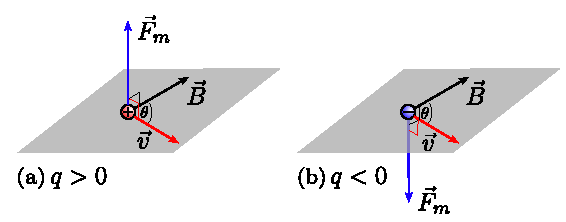
\includegraphics[scale = 1.4]{Figuras/Fuerza-Magnetica.pdf}
    \caption{Fuerza magnética para una carga positiva (a) y negativa (b).}
    \label{fig:Fuerza-Magnetica}
\end{figure}

La unidad de medida del campo magnético es el \textit{Tesla} ($T$), donde
$$1 \,[T] = 1 \, \left[ \frac{N s}{C m } \right] = 1 \,\left[ \frac{N}{A  m } \right].$$

Como la fuerza magnética se expresa con un producto cruz, el vector $\vec{F}_m$ es perpendicular a $\vec{v}$ y a $\vec{B}$. Además, la magnitud de la fuerza magnética sobre la carga es 
$$F_m = |q| vB \sin \theta,$$

donde $\theta$ es el menor ángulo que se forma entre $\vec{v}$ y $\vec{B}$. Luego, es inmediato ver que: la fuerza es nula si $\vec{v} \parallel \vec{B}$ y máxima cuando $\vec{v} \perp \vec{B}$.

\textbf{Observación:} Dado que la fuerza magnética y la velocidad de la carga son perpendiculares, tenemos que el \textit{campo magnético no realiza trabajo sobre la carga}. En consecuencia, el campo magnético sólo puede cambiar la dirección de la velocidad de una carga y no su módulo (energía cinética). \footnote{Recordar el teorema del trabajo y la energía: $W_{ab} = \int_a^b \vec{F} \cdot d\vec{x} = E_k(b) - E_k(a)$.}

Si sumamos la fuerza eléctrica y la magnética, obtenemos la \textbf{fuerza de Lorentz}:
\begin{shaded}
    $$\vec{F} = q (\vec{E} + \vec{v} \times \vec{B}).$$
\end{shaded}

\section{Aplicaciones de la fuerza de Lorentz}

Analizaremos tres problemas los cuales se aplicará lo estudiado en la sección anterior más conocimientos básicos de la mecánica newtoniana.

\begin{ejemplo}[Ciclotrón]
    Consideremos una carga puntual $q$ de masa $m$ que se mueve con una velocidad constante $\Vec{v}$. En cierto instante se ``prende'' un campo magnético uniforme $\Vec{B}$ perpendicular a la velocidad. Describa el movimiento de la carga $q$. 

\textbf{Solución:} Por regla de la mano derecha, notamos que el campo magnético produce una fuerza $\Vec{F}$ de tal forma que la velocidad de la carga cambia de dirección describiendo un movimiento circular uniforme (no cambia el módulo de la velocidad), para una demostración más rigurosa consulte el apéndice \ref{Mov-B-cte}.  

Si consideremos el sistema coordenado dado en la figura \ref{fig:Ciclotron} con $\Vec{B} = -B\,\hat{k}$, aplicando la segunda ley de Newton en coordenadas polares,
\begin{equation}
 \Vec{F} = q\vec{v} \times \vec{B} = m \frac{v^2}{r} (-\hat{r}), \label{Ciclotron-1}   
\end{equation}

donde $\Vec{a}_c = - m \frac{v^2}{r} \,\hat{r}$ es la aceleración centrípeta.

\begin{figure}[H]
    \centering
    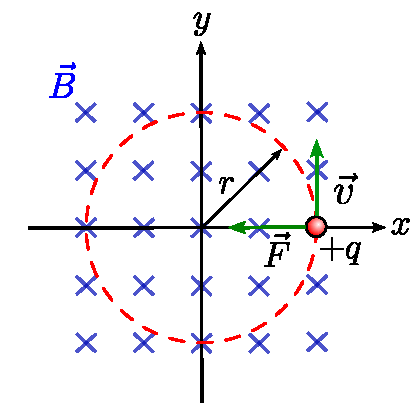
\includegraphics[scale = 1]{Figuras/Ciclotron.pdf}
    \caption{Ciclotrón}
    \label{fig:Ciclotron}
\end{figure}

En el instante inicial, 
$$\Vec{v} = v \,\hat{\jmath} ~~\text{y}~~ \Vec{a}_c = -  m \frac{v^2}{r} \,\hat{\imath}.$$

Reemplazando en \eqref{Ciclotron-1},
$$(q v\,\hat{\jmath}) \times (-B \,\hat{k}) = - m \frac{v^2}{r} \,\hat{\imath} \Rightarrow qvB = m \frac{v^2}{r}.$$

Entonces, el radio de curvatura es
\begin{equation*}
\boxed{r = \frac{mv}{qB}}
\end{equation*}

Recordemos que para el movimiento circular uniforme, la rapidez angular está dada por $\omega = v/r$. En nuestro caso,
\begin{equation*}
\boxed{\omega = \frac{qB}{m}}
\end{equation*}

Además,
\begin{equation*}
\boxed{f = \frac{\omega}{2\pi} = \frac{qB}{2\pi m}}
\end{equation*}

La expresión anterior se conoce como la \textbf{frecuencia de ciclotrón}. Es una característica de una partícula moviéndose en un campo magnético determinado.

\textbf{Observación:} En el caso que la velocidad de la carga puntual $q$ no sea perpendicular al campo magnético, el movimiento resultante es helicoidal. En efecto, si descomponemos la velocidad en una componente perpendicular al campo $\Vec{v}_{\perp}$ y otra componente paralela al campo $\Vec{v}_{\parallel}$, tal que $\Vec{v} = \vec{v}_{\perp} + \Vec{v}_{\parallel}$. Las ecuaciones para $\Vec{v}_{\perp}$ son las mismas del ciclotrón, pero para $\Vec{v}_{\parallel}$ se obtiene un movimiento rectilíneo uniforme a lo largo del campo. Por lo tanto, el movimiento resultante es la composición del movimiento en cada componente dando como resultado una helicoide, ver figura \ref{fig:Helicoide}.

\begin{figure}[H]
    \centering
    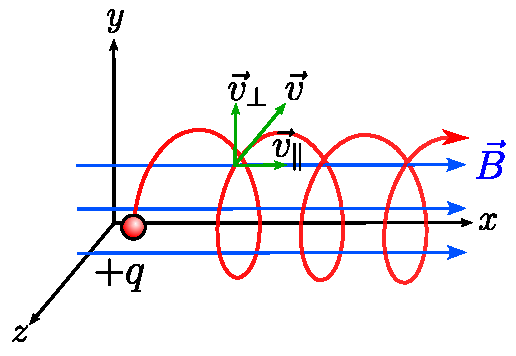
\includegraphics[scale = 0.9]{Figuras/Helicoidal.pdf}
    \caption{Carga puntual en un campo magnético uniforme con velocidad no perpendicular al campo.}
    \label{fig:Helicoide}
\end{figure}
\end{ejemplo}

\begin{ejemplo}[Selector de velocidades]
Queremos encontrar un método que nos permita seleccionar partículas cargadas con cierta velocidad dado un campo eléctrico  y magnético.

Supongamos que tenemos una partícula de carga $q$ que se mueve con una velocidad $\vec{v}$ en presencia de un campo magnético $\vec{B}$ y eléctrico $\vec{E}$ tal como se indica en la  figura \ref{fig:Selector-Velocidades}.

\begin{figure}[H]
    \centering
    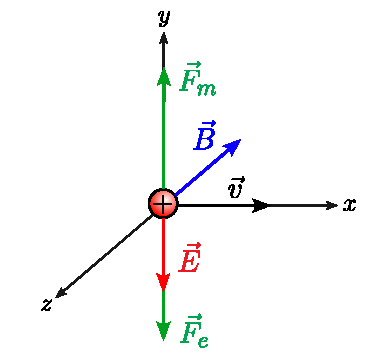
\includegraphics[scale = 0.9]{Figuras/Selector-Velocidades.pdf}
    \caption{Selector de velocidades.}
    \label{fig:Selector-Velocidades}
\end{figure}

Si ajustamos los campos eléctrico y magnético para que la fuerza de Lorentz se anule y así $\vec{v} = cte$ (la partícula no dobla).
$$\Vec{F}_e + \Vec{F}_m = -qE \,\hat{\jmath} + qvB \,\hat{\jmath} = \vec{0} \Rightarrow qE = qvB.$$

Entonces,
\begin{equation*}
\boxed{v = \frac{E}{B}}
\end{equation*}


\textbf{Conclusiones:}

\begin{enumerate}
\item Para seleccionar las partículas con rapidez $v$ es necesario ajustar los campos tal que $v = \frac{E}{B}$.

\item El valor $v$ es independiente de la carga y de la masa.
\end{enumerate}
\end{ejemplo}

\begin{ejemplo}[Selector de masas]
   
Ahora, no solo nos interesa un mecanismo para seleccionar  partículas con cierta velocidad, sino también su masa. Para ello se sigue el esquema de la figura \ref{fig:Selector-Masas}. En (a) se ajustan los valores del campo eléctrico $\Vec{E}$ y el campo magnético $\Vec{B}$, para seleccionar las partículas que posean una cierta velocidad $\Vec{v}$ tal que $v = E/B$. Una vez seleccionada la velocidad, éstas se hacen pasar por otra zona (b), donde sólo hay un campo magnético $\Vec{B}\,'$.

\begin{figure}[H]
    \centering
    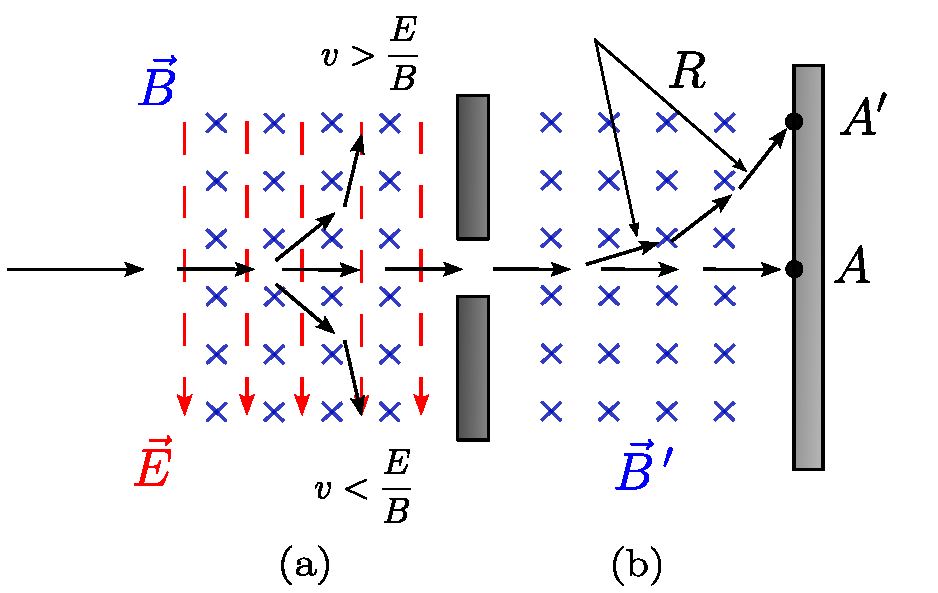
\includegraphics[scale = 0.7]{Figuras/Selector-Masas.pdf}
    \caption{Selector de masas.}
    \label{fig:Selector-Masas}
\end{figure}

Según lo visto en el ejemplo del ciclotrón, las partículas se desviarán siguiente una trayectoria circular con radio 
\begin{equation*}
\boxed{R = \frac{mv}{qB'}}
\end{equation*}

 Las partículas al ser pasadas por otro campo magnético (ajustable), algunas describen trayectorias circulares, donde el radio solo depende de la masa, obteniéndose así un selector de masas.
\end{ejemplo}

\section{Efecto Hall}

El \textbf{efecto Hall} consiste en la deflexión que experimentan los portadores de carga cuando fluyen por un conductor delgado sumergido en un campo magnético.

Consideremos una cinta conductora en un campo eléctrico estacionario $\Vec{E}$ en la dirección del eje $y$ y un campo magnético $\vec{B}$ uniforme y perpendicular al plano (en la dirección del eje $x$), ver figura \ref{fig:Efecto-Hall}. Se puede deducir una expresión que permite calcular la concentración efectiva y el tipo de portadores de carga.

\begin{figure}[H]
    \centering
    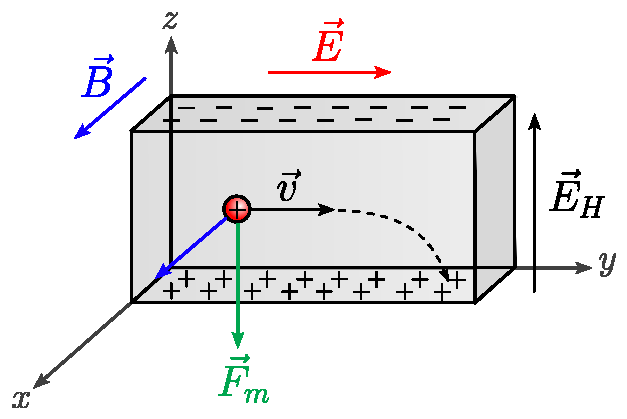
\includegraphics[scale = 0.8]{Figuras/Efecto_Hall.pdf}
    \caption{Efecto Hall.}
    \label{fig:Efecto-Hall}
\end{figure}

Supongamos que la corriente se debe al movimiento de portadores de carga positivos con carga $q$, entonces sobre ellos actúa una fuerza magnética
$$\vec{F}_m = q\vec{v} \times \vec{B},$$

la cual cual deflecta las cargas a la parte inferior del conductor. Así, dicho borde queda cargado positivamente y como la cinta es neutra, el borde de la parte superior queda cargado negativamente.

Estas cargas crean un campo electrostático llamado \textbf{campo de Hall}, que establece una condición de equilibrio para los portadores:
$$\vec{F}_m  + \vec{F}_e = \vec{0} \Rightarrow q(\vec{v} \times \vec{B} + \vec{E}_H) = \vec{0}.$$

Entonces,
$$\vec{E}_H = - \vec{v} \times \vec{B}.$$

Si $n$ es la densidad de portadores de carga por unidad de volumen, la densidad de corriente está dada por
$$\vec{J} = qn \vec{v} \Rightarrow \vec{v} = \frac{1}{qn} \vec{J}.$$

Definimos el \textbf{coeficiente de Hall} como
\begin{shaded}
    $$R_H = \frac{1}{qn}.$$
\end{shaded}

De esta manera, podemos reescribir el campo de Hall de la siguiente forma.
\begin{shaded}
    $$\Vec{E}_H = - \Vec{v} \times \Vec{B} = -R_H \Vec{J} \times \Vec{B}.$$
\end{shaded}

Para el sistema de referencia de la figura \ref{fig:Efecto-Hall}, tenemos que
$$\vec{E}_H = - R_H (J\, \hat{\jmath} \times B \,\hat{\imath}) = R_H JB  \,\hat{k}.$$

Ahora definimos el \textbf{voltaje de Hall} como la diferencia de potencial desde $z = 0$ hasta $z = h$.
\begin{align*}
    V_H &= \int_0^h \vec{E}_H \cdot d\vec{x} \\
&= \int_0^h (R_H JB  \hat{k}) \cdot (dz \,\hat{k}) \\
&=\int_0^h R_H JB  \,dz \\
&= R_HJB h.
\end{align*}

Como la intensidad de corriente está dada por
$$I = \iint_S \Vec{J} \cdot d\Vec{S} = \int_0^w \int_0^h (J \,\hat{\jmath})  \cdot (dz \,dx \, \hat{j}) = J wh \Rightarrow J = \frac{I}{wh},$$

donde $w$ es el ancho de la cinta conductora y $h$ el alto.

Reemplazando en $V_H$:
\begin{shaded}
    $$V_H = R_H \frac{IB}{w}.$$
\end{shaded}

En los experimentos, se puede posicionar un voltímetro para medir esta diferencia de potencial, lo cual es de útil para saber en verdad si son los portadores positivos o negativos los que se mueven, pues

\begin{itemize}
\item Si $V_H >0$ los portadores son positivos.

\item Si $V_H < 0$ los portadores son negativos.
\end{itemize}

\section{Fuerza magnética sobre un conductor con corriente}

Vimos que existe una fuerza sobre una carga en movimiento en presencia de un campo magnético. Ahora determinaremos la fuerza sobre un conductor, ver figura \ref{fig:Fm-Conductor}.

\begin{figure}[H]
    \centering
    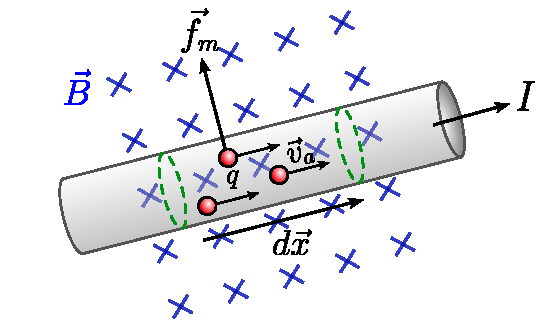
\includegraphics[scale = 0.95]{Figuras/Fuerza-Magnetica-Conductor.pdf}
    \caption{Fuerza magnética sobre un conductor.}
    \label{fig:Fm-Conductor}
\end{figure}

Si en un campo magnético $\vec{B}$ existe un alambre por el que fluye una corriente $I$, cada una de las cargas en movimiento experimenta una fuerza magnética dada por
$$\vec{f}_m = q \vec{v}_a \times \vec{B},$$

donde $\vec{v}_a$ es la velocidad de arrastre de la carga $q$.

Si $n$ es el número de portadores de carga móviles por unidad de volumen (densidad de portadores de carga), entonces la fuerza sobre un segmento de conductor de largo $dx$ y sección transversal $A$, ésta dada por
$$d\Vec{F}_m = n q (A dx) \Vec{v}_a \times \Vec{B}.$$

Como la corriente (para un conductor recto) se puede escribir $I = J A = n q A v_a$, tenemos que
$$d\vec{F}_m = (nAqv_a)(dx \,\hat{v}_a) \times \vec{B} = I (dx\, \hat{v}_a) \times \vec{B} = I d\vec{x} \times \vec{B}.$$

Por lo tanto, la fuerza ejercida sobre un alambre conductor con corriente $I$ en presencia de un campo magnético $\Vec{B}$, es
\begin{shaded}
    $$\Vec{F}_m = \int_a^b I \,d\Vec{x} \times \Vec{B},$$
\end{shaded}

donde $a$ y $b$ representan los extremos del conductor.

\textbf{Caso particular:} Para un alambre recto de longitud $L$ que circula una corriente $I$ sumergido en un campo uniforme $\vec{B}$, la fuerza magnética sobre él es

\begin{equation*}
\vec{F}_m = I \vec{L} \times \vec{B}.
\end{equation*}

En general, si las cargas están distribuidas continuamente, entonces la fuerza magnética total sobre un volumen $V$ con densidad $\rho$ y velocidad $\Vec{v}$ será
 \begin{shaded}
 $$\vec{F}_m = \iiint_V \rho \Vec{v} \times \Vec{B} \,dV = \iiint_V  \Vec{J} \times \Vec{B} \,dV.$$    
 \end{shaded}

\subsection{Aplicación: Torque sobre una espira}

Consideremos una espira rectangular en el plano $xz$ de lados $a$ y $b$ por la cual fluye una corriente $I$ con el sentido de la figura \ref{fig:Espira}. Determinemos el torque que un campo magnético uniforme en la dirección del eje $x$ ejerce sobre la espira.

\begin{figure}[H]
    \centering
    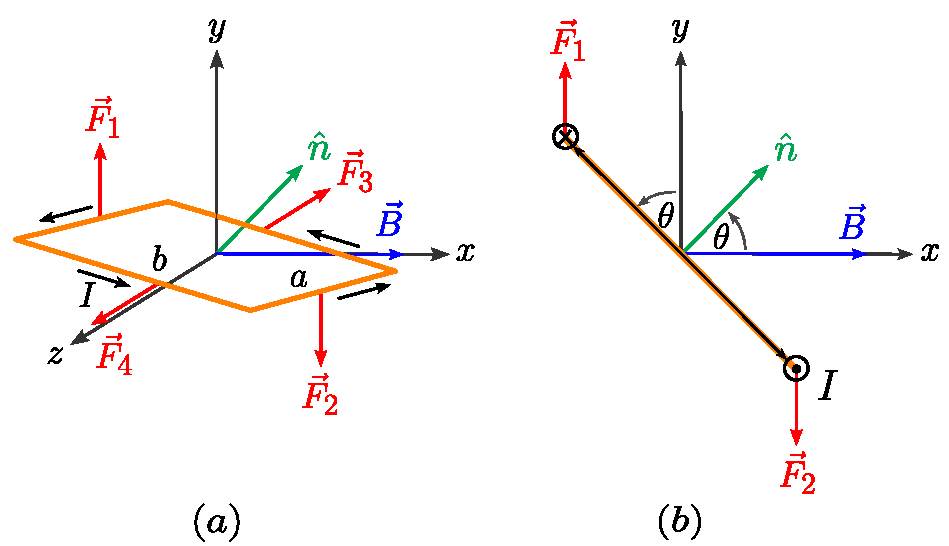
\includegraphics[scale = 0.8]{Figuras/Espira.pdf}
    \caption{Espira rectangular con corriente $I$ rotando sobre el eje $z$ producto de un campo magnético uniforme $\Vec{B}$ en (a) y su proyección sobre el plano $xy$ en (b).}
    \label{fig:Espira}
\end{figure}

Producto del campo magnético, la espira rotará quedando Los lados de longitud $a$ del rectángulo paralelos al eje de rotación (eje $z$).

Recordemos que para este caso particular, la fuerza sobre cada lado de la espira está dada por
$$\vec{F} = I \vec{L} \times \vec{B}.$$


Entonces, las fuerzas que actúan en la espira son:
\begin{align*}
 \vec{F}_1 &= I (a \,\hat{k}) \times (B \,\hat{\imath}) = IaB \,\hat{\jmath}, \\
\vec{F}_2 &= I (-a \,\hat{k}) \times (B\, \hat{\imath}) = -IaB \,\hat{j}, \\
\vec{F}_3 &= I (b \sin\theta \,\hat{\imath} - b \cos\theta \,\hat{\jmath}) \times (B \,\hat{\jmath}) = Ib \sin \theta B \,\hat{k}, \\
\vec{F}_4 &= I (-b \sin \theta \,\hat{\imath} + b \cos \theta \,\hat{\jmath}) \times (B\, \hat{j}) = -Ib \sin \theta B \,\hat{k}.   
\end{align*}

De inmediato vemos que
$$\sum \vec{F} = \vec{F}_1 + \vec{F}_2 + \vec{F}_3 + \vec{F}_4 = \vec{0}.$$

Por lo tanto, no hay movimiento traslacional, pero sí rotacional, debido a que las fuerzas $\vec{F}_1$ y $\vec{F}_2$ producen torque.

Considerando
\begin{align*}
\vec{x}_1 &= \frac{b}{2} \cos \left( \theta + \frac{\pi}{2} \right) \hat{\imath} + \frac{b}{2} \sin \left(\theta + \frac{\pi}{2} \right) = \frac{b}{2} (- \sin \theta \,\hat{\imath} + \cos\theta \,\hat{\jmath}), \\
\vec{x}_2 &= - \vec{x}_1 = \frac{b}{2} (\sin \theta \,\hat{\imath} - \cos\theta \,\hat{\jmath}),    
\end{align*}

el torque neto con respecto al origen del sistema está dado por
\begin{align*}
\vec{\tau} &= \vec{x}_1 \times \vec{F}_1 + \vec{x}_2 \times \vec{F}_2 \\
&= \frac{b}{2} (- \sin \theta \,\hat{\imath} + \cos\theta \,\hat{\jmath}) \times (IaB \,\hat{\jmath}) +\frac{b}{2} (\sin \theta \,\hat{\imath} - \cos\theta \,\hat{\jmath}) \times (-IaB \,\hat{\jmath}) \\
&= -IaB \frac{b}{2} \sin \theta\, \hat{k} - IaB \frac{b}{2} \sin \theta \,\hat{k} \\
&= - IabB \sin \theta \,\hat{k} \\
&= -I AB \sin \theta \,\hat{k},    
\end{align*}


donde $A$ es el área de la espira.

Si definimos el \textbf{momento dipolar magnético} como 
\begin{shaded}
    $$\Vec{\mu} = I \vec{A} = IA \,\hat{n},$$
\end{shaded}

donde $\hat{n}$ es el vector unitario normal a la superficie limitada por la esfera.

El torque neto nos queda
\begin{shaded}
    $$\vec{\tau} = \vec{\mu} \times \vec{B}.$$
\end{shaded}

En efecto, a partir de la figura \ref{fig:Espira}, tenemos que
$$\hat{n} = \cos \theta \,\hat{\imath} + \sin\theta \,\hat{\jmath}.$$

Luego,
\begin{align*}
   \vec{\tau} = \vec{\mu} \times \vec{B} &= (IA \,\hat{n}) \times (B\,\hat{\imath}) \\
   &= IA B (\cos \theta \,\hat{\imath} + \sin  \theta \,\hat{\jmath}) \times \hat{\imath} \\
   &= - IAB \sin \theta\,\hat{k}.
\end{align*}

\textbf{Observación 1:} Este resultado se puede generalizar para una espira de cualquier otra forma.

\textbf{Observación 2:} Lo expuesto corresponde a los principios del funcionamiento de un motor eléctrico. \footnote{En el siguiente \href{https://youtu.be/24lasu4V8NI}{link} se encuentra alojado un vídeo con una animación que ilustra el funcionamiento de un motor eléctrico.}

\section{Ley de Biot-Savart}

\section{Potencial vectorial y ley de Gauss para el magnetismo}

\subsection{Potencial vectorial*}

\subsection{Ley del Gauss para el magnetismo}

\section{Ley de Ampère}

\section{Campo magnético en la materia}



